\section{Event Selection and Categorization}\label{sec:selection}

Signal events are selected on the basis of large values of \ETm and one or more high-\pt jet(s), 
explicitly vetoing isolated leptons and photons. The data used for this analysis are collected using two triggers designed to record events that 
contain a large \ETm. The first requires events for which \ETm, calculated using only information from the calorimeters, is larger 
than 120 \gev. The second trigger is a dedicated monojet trigger which selects events 
based on the amount of \ETm reconstructed using the online version of the particle-flow algorithm. Identified muons are 
removed from the event before the \ETm is calculated so that $\Zmm$ events are also selected. These events are   
used as a control sample for the $\Zvvjets$ background as described in Section~\ref{sec:zjetsmodel}. The \ETm threshold for the second trigger is 95 GeV. 
The \ETm threshold of this trigger is 95~\gev and 105~\gev for the first and second half of the 2012 
data-taking period respectively. The threshold on the \ETm for the selection of the events 
is set at 200 \gev in order to maintain a high efficiency from the triggers.
In addition, for the second trigger, the event is required to contain a jet with \pt$>80$ \gev and $|\eta|<2.6$ for 
which no more than 95\% of the jet's energy is associated to neutral hadrons. The efficiency of these triggers 
is greater than $99$\% with respect to the full event selection. 

Jets are obtained from the clustering of PF objects 
by means of either the anti-$k_{\textrm{T}}$ algorithm~\cite{Cacciari:2008gp} with 0.5 (ak5 jet) as the distance parameter,  
or the Cambridge/Aachen algorithm~\cite{cajets} with 0.8 distance parameter (ca8). 
Further selections are applied on the leading jet based
on the fractions of energy associated to the PF candidate types to reduce the contribution from 
anomalous energy measurements. Namely, the charged hadrons fraction has to be larger than 0.2, 
the neutral electromagnetic fraction has to be smaller than 0.7 
and the neutral hadronic fraction has to be smaller than 0.7.
Jet energies are corrected for pileup on the basis of the event energy density and 
proportionally to their area. Data-driven scale calibrations are then applied to correct the energy of the 
jets~\cite{jec}.

The \ETm is calculated as the magnitude of the negative 
vector sum of the transverse momenta of all final state particles, which are reconstructed 
using the particle-flow (PF) algorithm~\cite{CMS-PAS-PFT-09-001}.
Events with a large mis-reconstructed offline \ETm are removed by applying quality filters. 
The angle between the \ETm and the leading jet is required to be larger than 2 to reduce the contribution from multijet QCD events. 
Finally, events are vetoed which contain at least one well-identified and isolated electron, photon or muon with $p_T>10$~\gev, or a tau with $p_T>15$~\gev.

Selected events are classified into three event categories, based on the topology of the jets, in order to distinguish between 
initial or final state radiation of gluons or quarks versus jets arising from hadronic vector boson decays.
Events are first scrutinized for the presence of an unresolved vector boson, subsequently for a resolved vector boson 
and finally the remaining events are collected into the monojet category.

%\subsection{Unresolved (Boosted) V-tagged category}\label{sec:resvtagging}
If the  electroweak boson decays hadronically and it has sufficiently high transverse momentum, both its hadronic
decay products are captured by a single reconstructed ``fat''-jet. 
The selection for this category is devised to identify such events by selecting events containing a ca8 jet with a large $\pt$. 
The variable ``N-subjettiness'', $\tau_N$, defined in~\cite{Thaler:2010tr,Thaler:2011gf}, 
has been shown to be a powerful discriminator for hadronic V-tagging when combined into ratios
$\tau_N/\tau_{N-1}$, where $N$ is the hypothesized number of subjets. For the boosted vector boson topology, the discriminating ratio is $\tau_2/\tau_1$.
Additionally, the jet mass is used as it is the most natural discriminator between jets originating 
from vector boson decays and those originating from single partons. The ca8 jet mass is recomputed using a jet 
grooming technique to improve mass resolution by reducing the effects from pileup and underlying event.
Events with $\ETm>250$ \gev and a ca8 jet with $\pt>200$ \gev are categorised as boosted if the 
jet additionally satisfies the criteria that the $\tau_2/\tau_1$ ratio is smaller than 0.5 and
the pruned jet mass~\cite{Ellis:2009me}, $m_{\mathrm{prune}}$, satisfies $60<m_{\mathrm{prune}}<110$ \gev.  
%Figure~\ref{fig:boostvtagvars} shows the distributions of $\tau_2/\tau_1$ and $m_{\mathrm{prune}}$, (before the application 
%of the jet mass cut) in simulation and data for the boosted event category. 
%\begin{figure*}[hbtp]\begin{center}
%\subfigure[]{
% 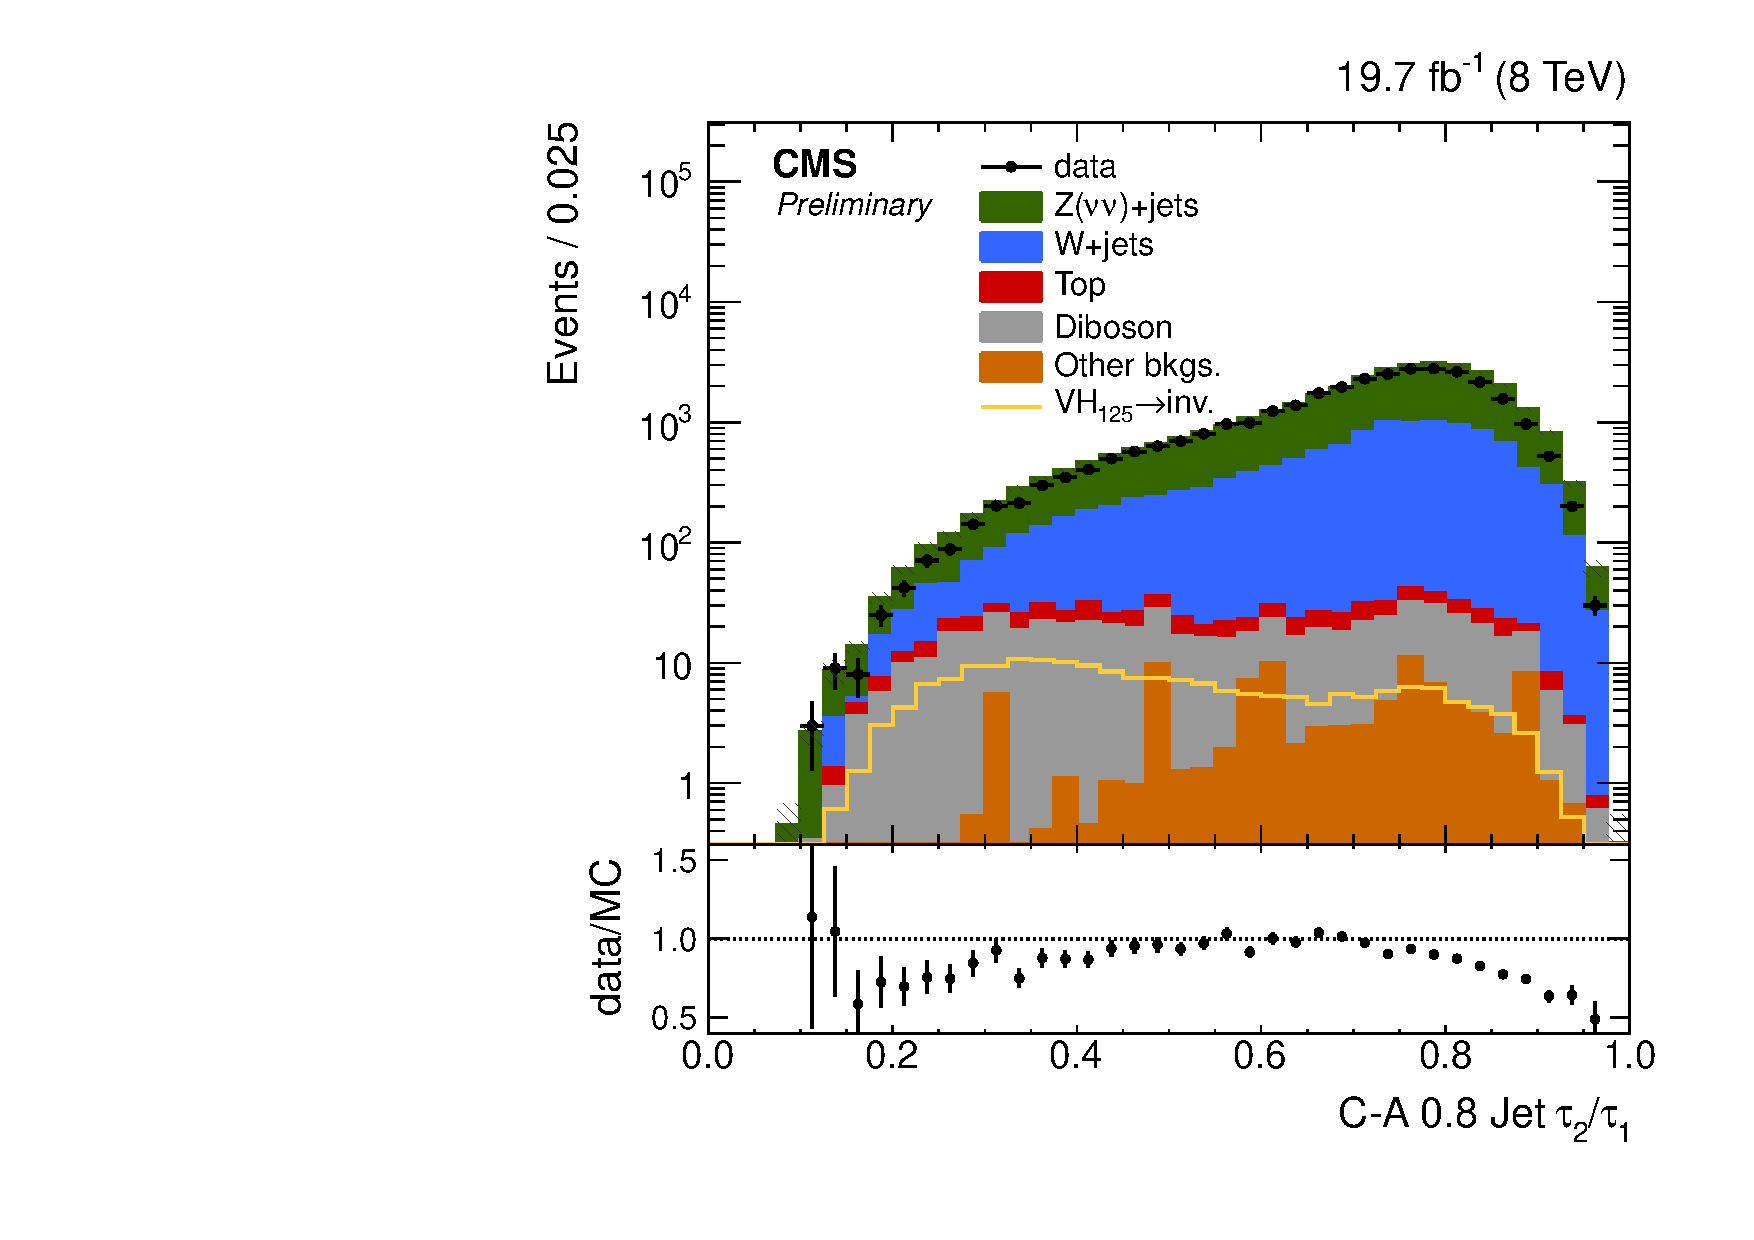
\includegraphics[width=0.49\textwidth]{fig/t2t1_sig_baseline.pdf}
%}
%\subfigure[]{
% 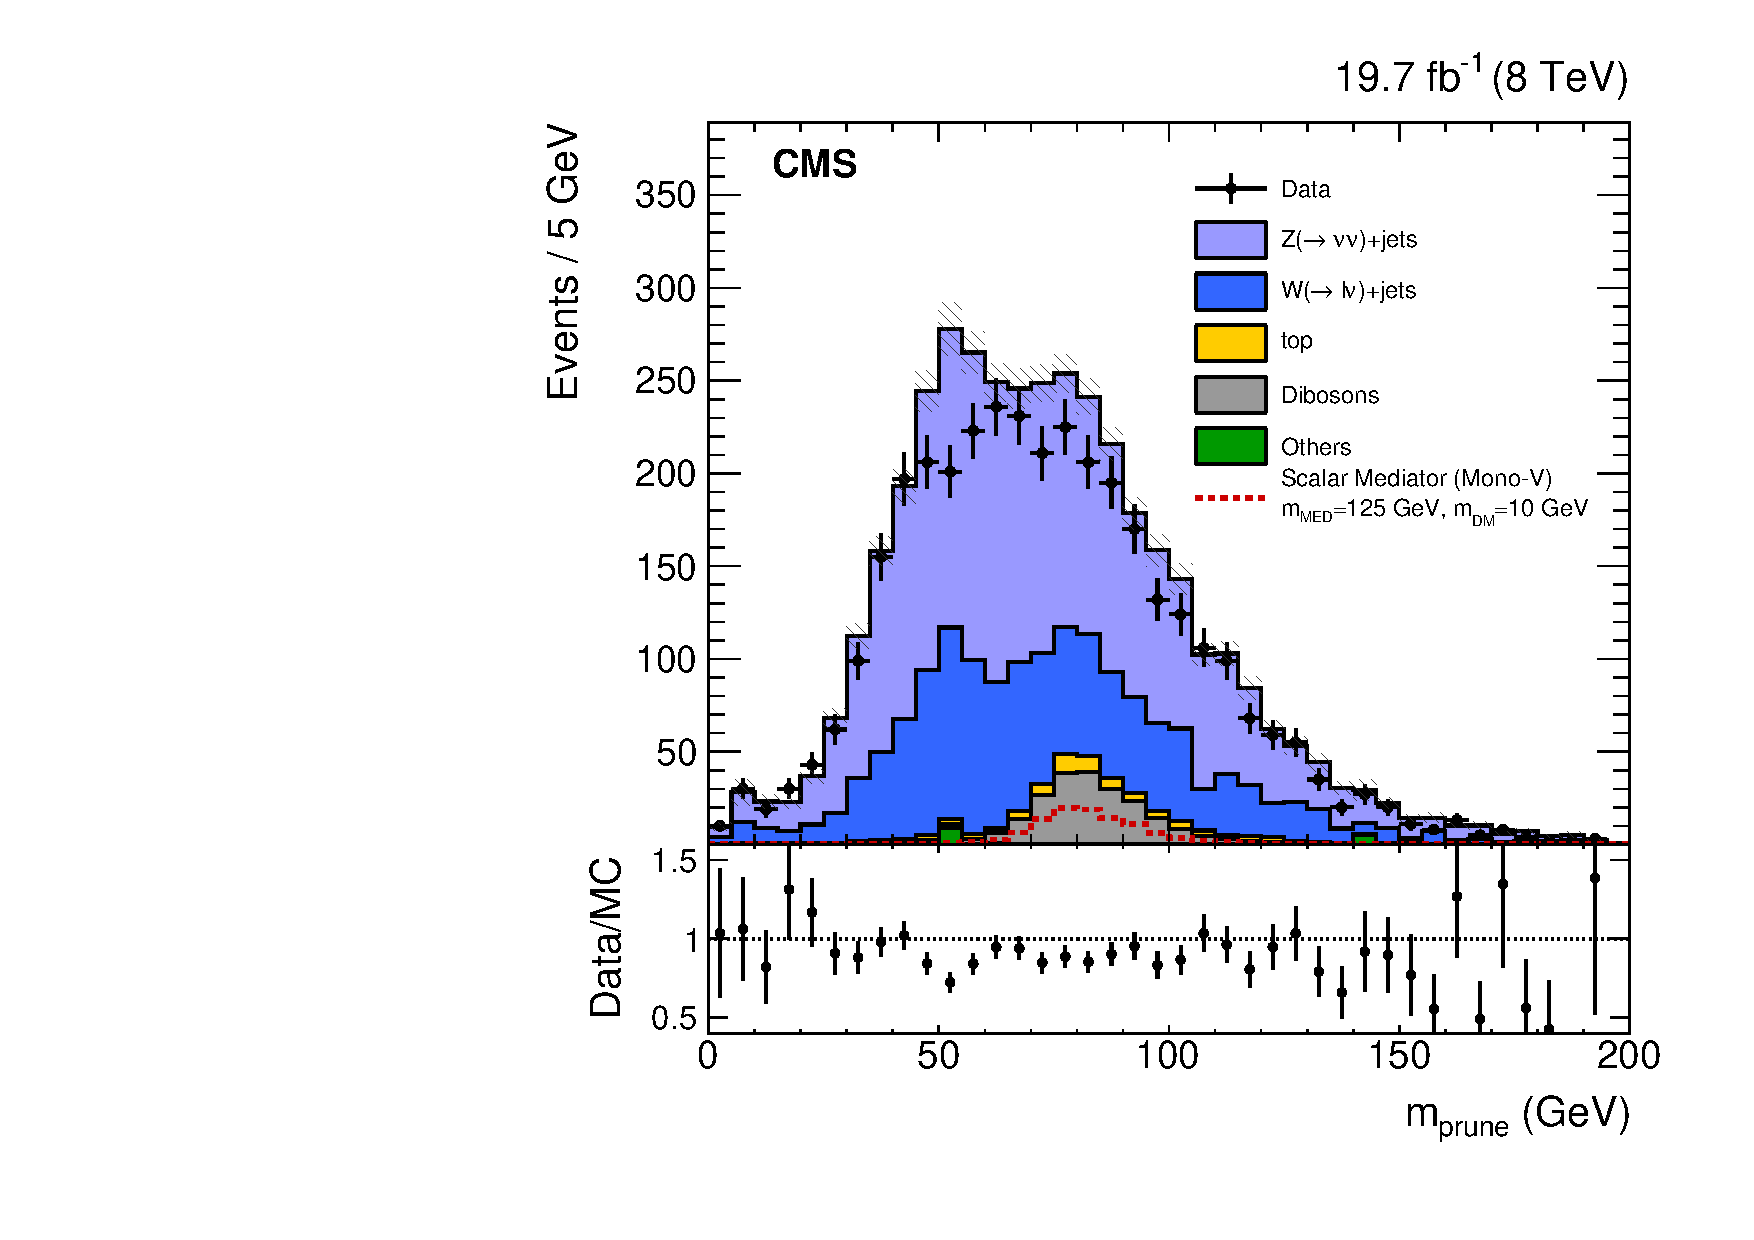
\includegraphics[width=0.49\textwidth]{fig/mass_sig_nomasscut.pdf}
%}
% \caption{Distributions of $\tau_2/\tau_1$ before the jet mass cut (a) and pruned jet mass (b) for events in data and MC in the boosted event category. 
% A cut of $\tau_2/\tau_1<$0.5 is applied in figure b.}
% \label{fig:boostvtagvars}\end{center}\end{figure*}

Events which contain additional jets close to the ca8 jet, but no closer than $\Delta R < 0.5$,
are selected to include the frequent cases in which initial state radiation yields additional jets. 
If an ak5 jet with $p_T>30$ and $|\eta|<2.5$ is reconstructed, and the opening angle between it 
and the ca8 jet, $\Delta\phi(\mathrm{ak5,ca8})$, is smaller than 2, the event is selected. Events with more than one ak5 jets 
with $p_T>30$ \gev and $|\eta|<2.5$, reconstructed at $\Delta R> 0.5$ with respect to the ca8 jet 
are rejected.

%\subsection{Resolved V-tagged category}\label{sec:resvtagging}
In cases where the electroweak boson has insufficient transverse momentum for its hadronic
decay to be fully contained in a single reconstructed fat-jet, a selection that looks for decays 
into a pair of ak5 jets is applied to recover the event. 
The selection requires that each jet has $p_T>30$ GeV and $|\eta|<2.5$ and that the dijet has a mass between 60\gev and 110\gev, consistent with originating 
from an electroweak boson.
After such a selection, there is still a large combinatorial background of random
pairing of jets from processes such as Z+jets and W+jets. To further reduce the combinatorial background, a
multivariate V-tagger is applied. The inputs to this resolved V-tagger are the values from each jet of likelihood-based discriminator variable 
which distinguishes quark-initiated jets from gluon-initiated jets~\cite{JME-14-002}, the jet pull angle~\cite{Gallicchio:2010sw} and the mass drop variable~\cite{Izaguirre:2014ira}.
%\begin{itemize}
%\item{\bf Quark/Gluon Discriminator.} A likelihood-based discriminator that distinguishes quark-initiated jets from 
%gluon-initiated jets. The discriminator value from both jets are provided as input to the V-tagger~\cite{JME-14-002}.
%\item{\bf Jet Pull Angle.} The jet pull angle~\cite{Gallicchio:2010sw} is correlated with the color connection of a pair of jets. Since electroweak bosons
%are color singlets, the jets from their decays tend to have a smaller pull angle, in contrast to the combinatorial background
%that have no preferred angle. The pull angle of the trailing jet with respect to the leading jet and vice versa are given
%as input to the V-tagger.
%\item{\bf Mass Drop.} The mass drop variable is defined as~\cite{Izaguirre:2014ira},
%\begin{displaymath}
%   \frac{\max\left(m_1,m_2\right)}{m_{12}}\Delta R_{12},
%\end{displaymath}
%where $m_1$ and $m_2$ are the masses of each jet, $m_{12}$ is the dijet mass, and $\Delta R_{12}$ is the separation between
%the jets. This quantity tends to be smaller for dijets from vector boson decays compared to random pairings from background.
%\item{\bf Dijet $p_T/m$.} Ratio of the dijet $p_T$ to the dijet mass. This variable was found to perform better than the 
%dijet $p_T$ alone.
%\end{itemize}

%The distribution of the V-tagger variable for SM backgrounds and a Higgs boson with mass of 125 \gev produced in association 
%with either a W or Z boson is shown in Figure~\ref{fig:vtagger}.
%\begin{figure*}[hbtp]\begin{center}
%  \subfloat[][]{
% 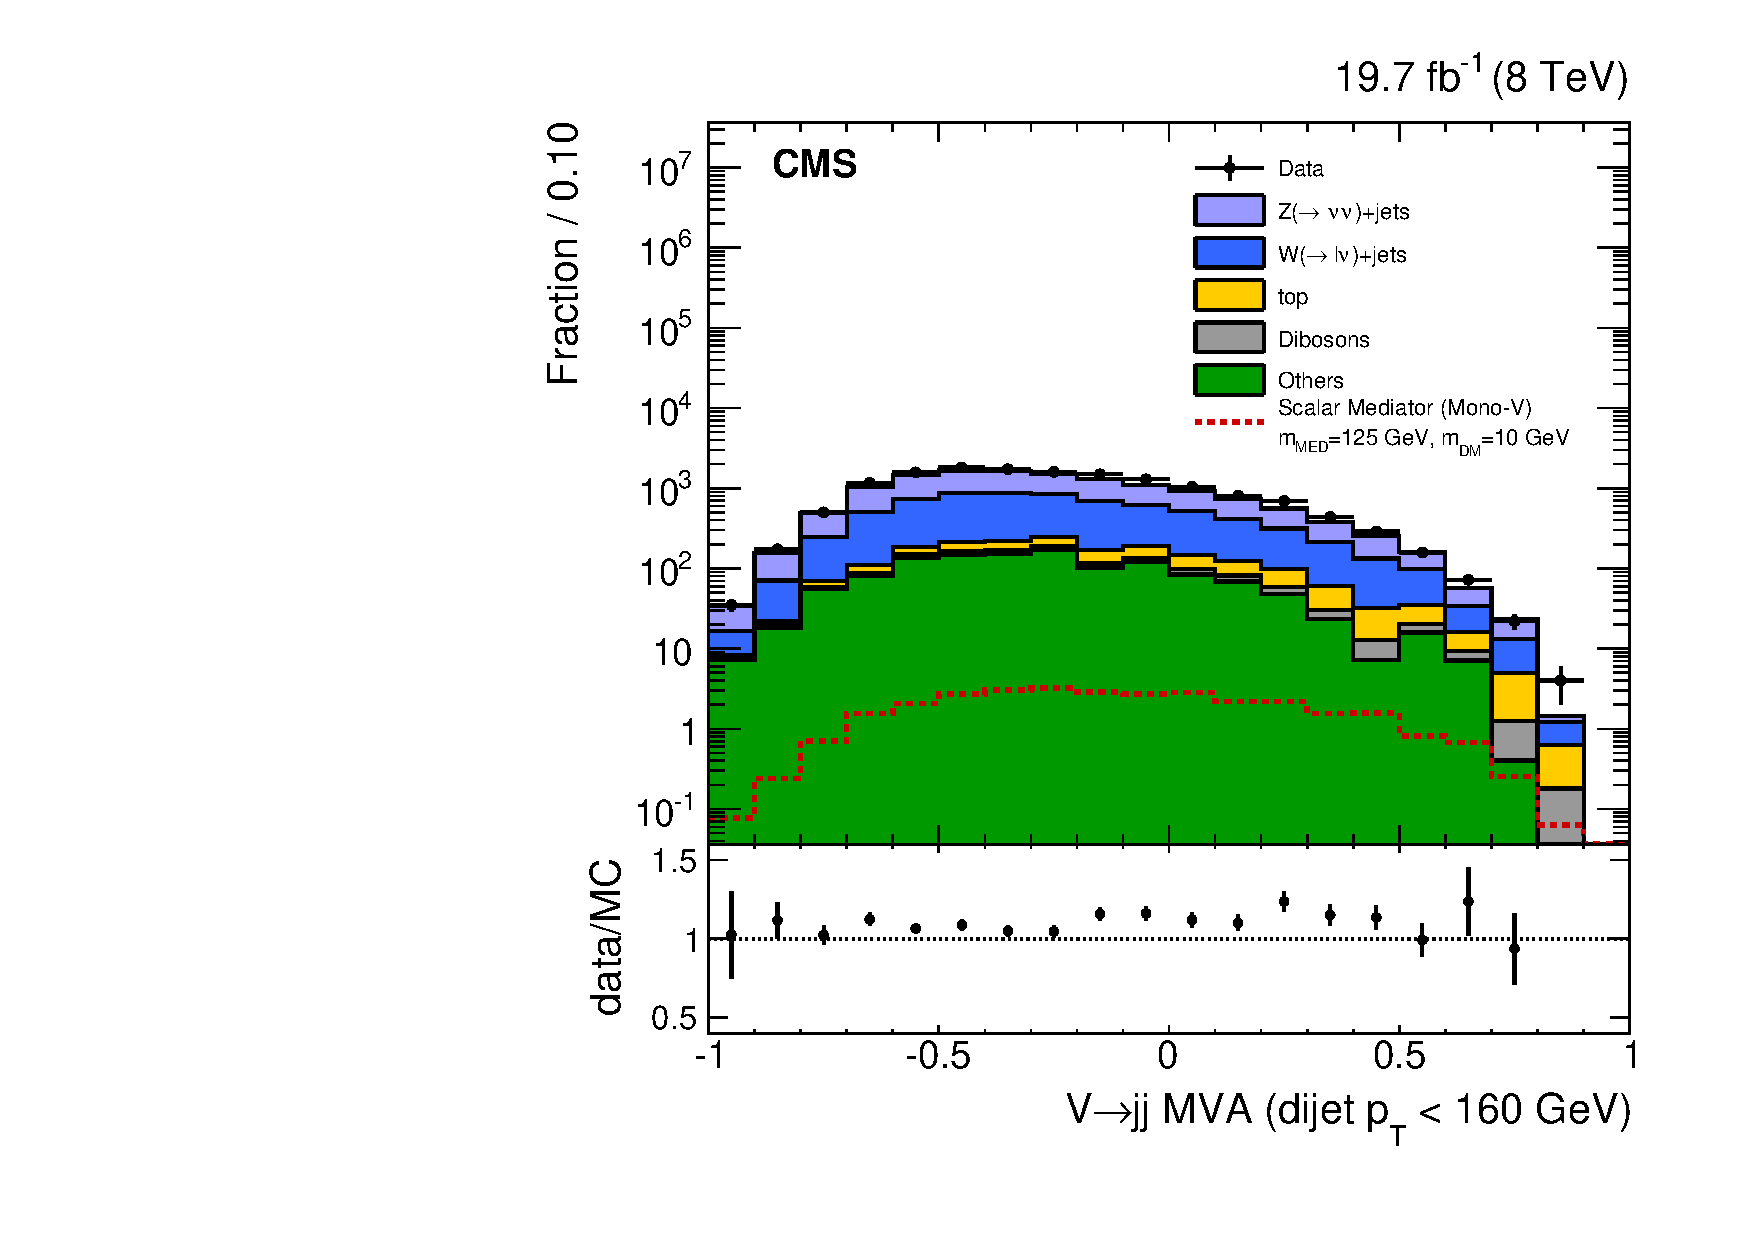
\includegraphics[width=0.49\textwidth]{fig/res_vmvalog_0.pdf}
%}
%  \subfloat[][]{
% 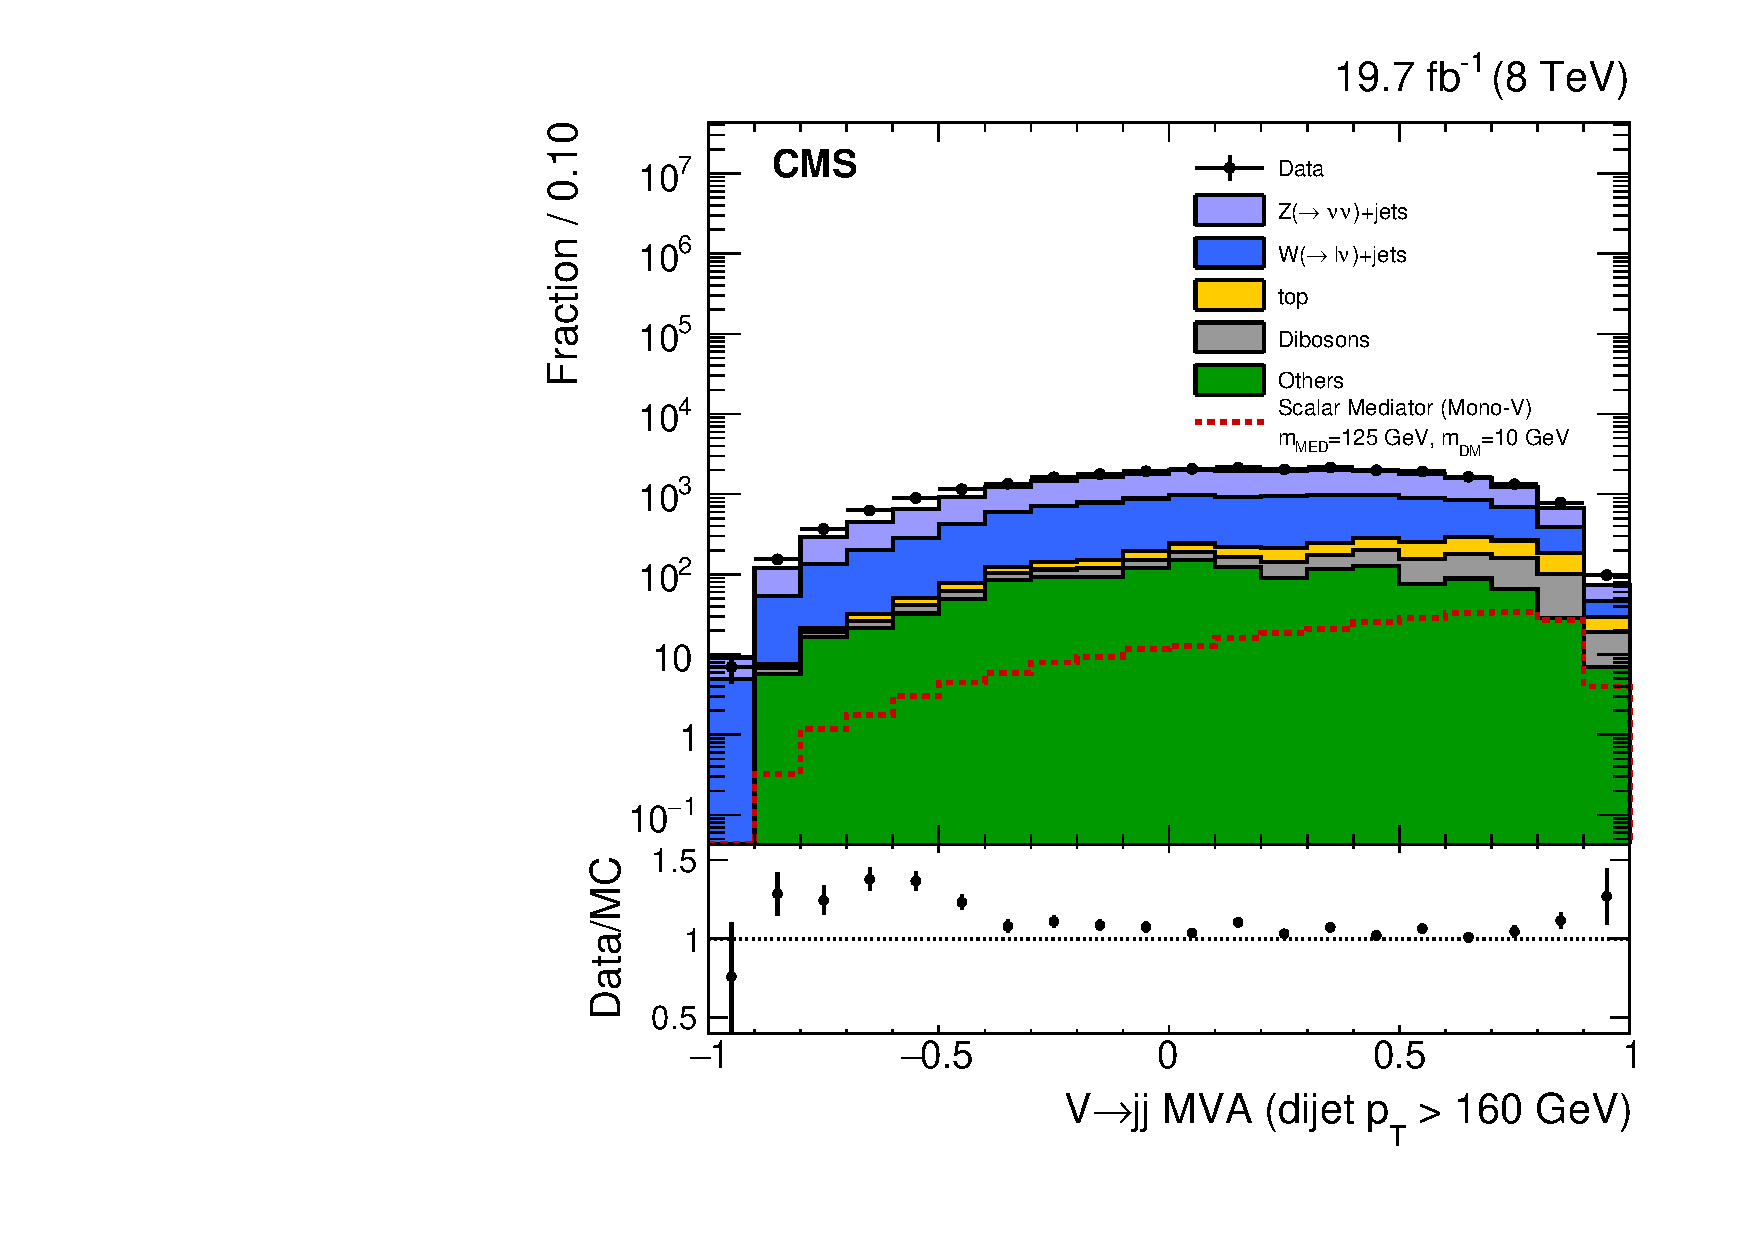
\includegraphics[width=0.49\textwidth]{fig/res_vmvalog_1.pdf}
%}
% \caption{
%Resolved V-tagger variable distribution in simulation and data after all other
%signal region cuts in the resolved category. 
%The distributions are shown split into dijet $\pt < 160$ \gev (a) and dijet
%$\pt > 160$ \gev (b), corresponding roughly to the point at which jets begin to overlap. 
%The expected distribution for the vector boson produced in association with a Higgs boson with a mass of 125 \gev is shown.} 
% \label{fig:vtagger}\end{center}\end{figure*}

To be tagged as a hadronic V-boson decay, the value of the discriminator for the event must be larger than 0.6. In events 
where multiple dijet pairs are found, the pair with the highest V-tagger value is taken as the candidate. 
To reduce contamination from top backgrounds, the event is rejected if it contains a 
b-tagged jet, defined using the CSV medium definition~\cite{BTAG}. Finally, the events are required to 
have $\ETm>250$ \gev to avoid the bias of the \ETm spectrum introduced from the requirements 
on the dijet system's transverse momentum through the application of the V-tagger.

The events that do not qualify for either of the two V-tagged categories are tested for the presence of a single jet originating from quark or gluon radiation. 
For the monojet category, at least one ak5 jet within $|\eta|<2.0$ with \pt greater 
than 150 \gev and a \ETm greater than 200 \gev is required.  
As in the boosted category, events with a second ak5 jet close to the leading one ($\Delta\phi(j_1,j_2) < 2$) 
with $p_T>30$ GeV and $|\eta|<2.5$ are selected to allow the frequent cases where initial state radiation yields two jets.
Events with three or more ak5 jets with $p_T>30$ \gev and $|\eta|<2.5$ are rejected.

Figure~\ref{fig:ptandmet} shows the \ETm and leading jet $p_{T}$ distributions in data and 
simulation after selection for all three event classes combined. The backgrounds are normalized to 19.7\fbinv 
and the expected distribution for vector mediated DM production assuming a DM mass of 10 GeV and mediator mass of 1 GeV is shown. 
The discrepancy between the data and simulation is a result of both mis-modelling of the 
detector resolution and an imperfect theoretical description of the kinematics of the W/Z+jet processes. 
Both effects are corrected for in this analysis using a data-driven approach described in the following section. 

\begin{figure*}[hbtp]\begin{center}
  \subfloat[][]{
 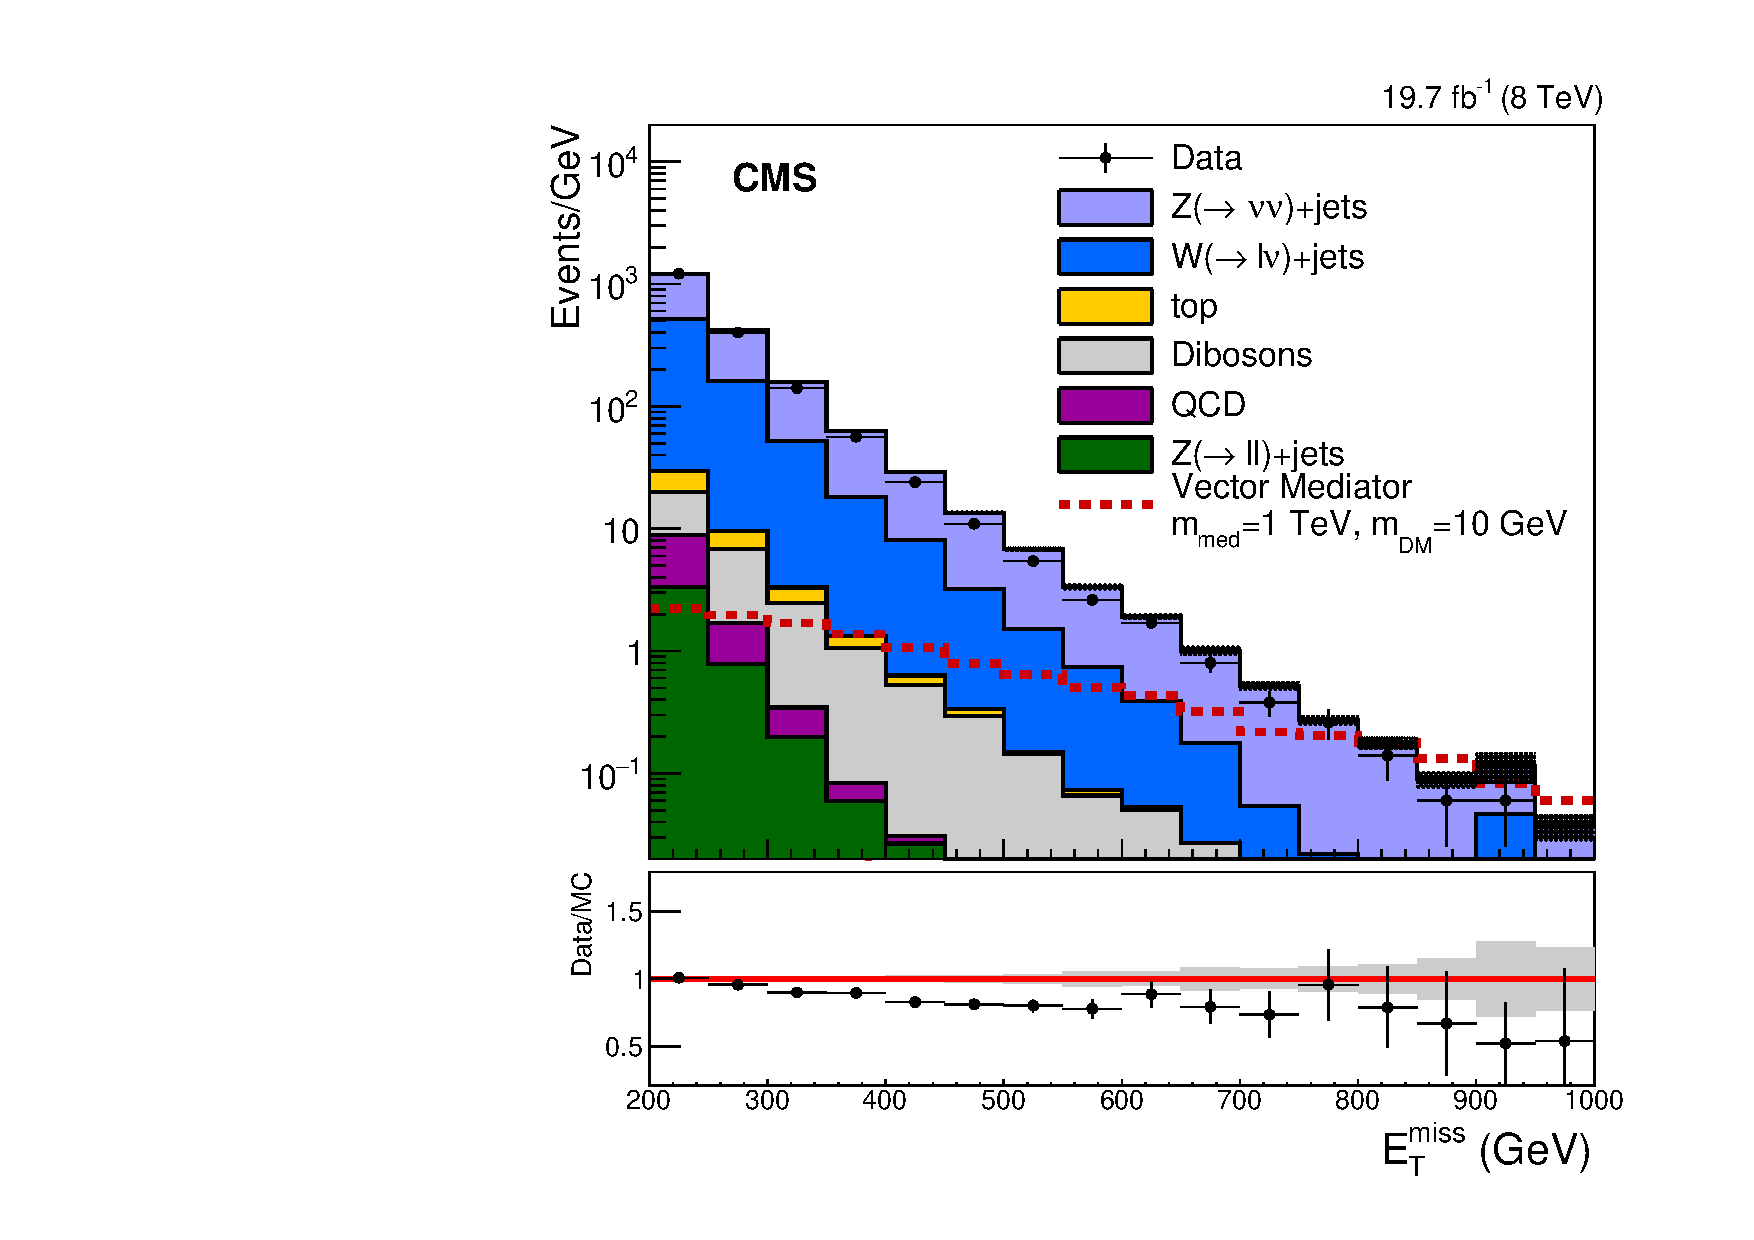
\includegraphics[width=0.49\textwidth]{figures/plot_config_combined_nocorr.pdf}
}
  \subfloat[][]{
 \includegraphics[width=0.49\textwidth]{figures/plot_config_combined_nocorr_jetPT.pdf}\\
}
 \caption{
   Distributions of \ETm (a) and leading jet $p_{T}$ (b) in simulated events and data after the signal selection for all three
   event categories combined. The dashed red line shows the expected distribution assuming vector mediated DM production with $m_{DM}=10$ GeV and $m_{MED}=1$ TeV.
   The gray band in the ratio panels indicate the statistical uncertainty from the limited number of background MC events.
 }
 \label{fig:ptandmet}\end{center}\end{figure*}



